\section{Hagan Rowlenstino A. S(1174040)}
\subsection{Instalasi Map Server}
\begin{enumerate}
    \item Download terlebih dahulu aplikasi mapservernya di ms4w.com . disini saya mendownload versi .exe nya agar lebih mudah dalam Instalasi
    \hfill\break
    \begin{figure}[H]
		
\includegraphics[width=12cm]{figures/1174040/Python3/exe.PNG}
		\centering
		\caption{File .exe ms4w}
	\end{figure}
    \item Pilih agree
    \hfill\break
    \begin{figure}[H]
		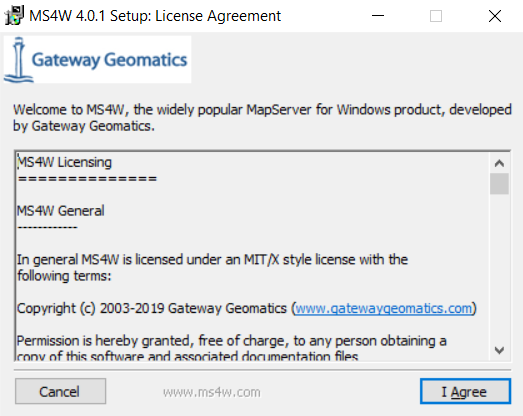
\includegraphics[width=12cm]{figures/1174040/Python3/1.PNG}
		\centering
		\caption{Pilih Agree}
	\end{figure}
    \item Check pilihan MapServer Itasca Demo Appllication dan biarkan yang lainnya seperti pada kondisi awal
    \hfill\break
    \begin{figure}[H]
		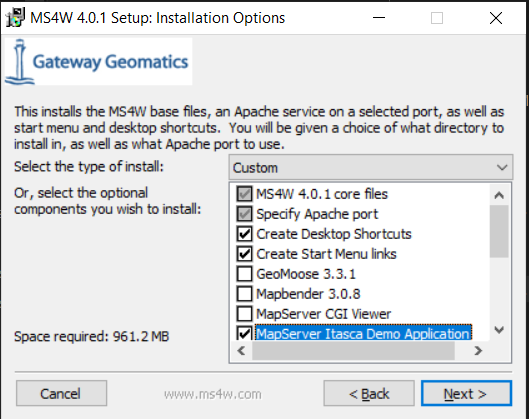
\includegraphics[width=12cm]{figures/1174040/Python3/2.PNG}
		\centering
		\caption{Pilih Itasca Demo Application}
	\end{figure}
    \item Pilih Directory
    \hfill\break
    \begin{figure}[H]
		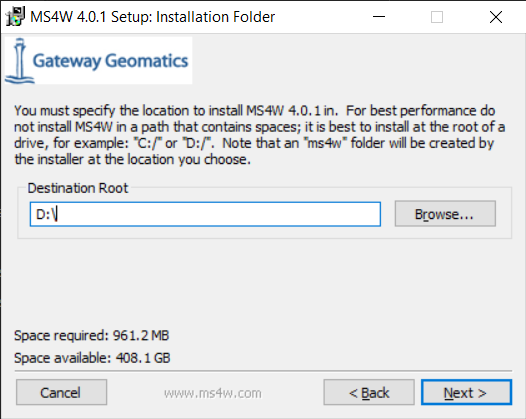
\includegraphics[width=12cm]{figures/1174040/Python3/3.PNG}
		\centering
		\caption{Pilih Directory}
	\end{figure}
    \item Pilih port mana yang akan digunakan, saya menggunakan port 82
    \hfill\break
    \begin{figure}[H]
		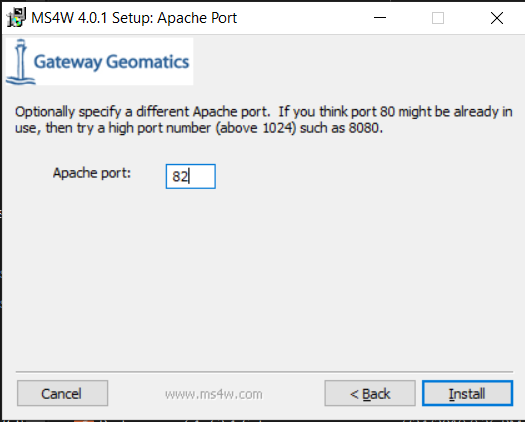
\includegraphics[width=12cm]{figures/1174040/Python3/4.PNG}
		\centering
		\caption{Pilih Port}
	\end{figure}
    \item Lalu tunggu sampai instalasi selesai
\end{enumerate}
\subsection{Instalasi Map Proxy}
\begin{enumerate}
    \item Kita ketikkan pip instal MapProxy di dalam command prompt
    \hfill\break
    \begin{figure}[H]
		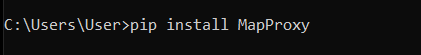
\includegraphics[width=12cm]{figures/1174040/Python3/5.PNG}
		\centering
		\caption{pip install mapproxy}
	\end{figure}
    \item Instal pyproj untuk berjaga - jaga apabila dibutuhkan dengan cara pip install pyproj
    \hfill\break
    \begin{figure}[H]
		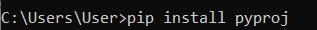
\includegraphics[width=12cm]{figures/1174040/Python3/6.PNG}
		\centering
		\caption{pip install pyproj}
	\end{figure}
    \item Download file yang telah disediakan oleh Pak rolly yang berada dalam file gede yang berisikan peta indonesia
    \hfill\break
    \begin{figure}[H]
		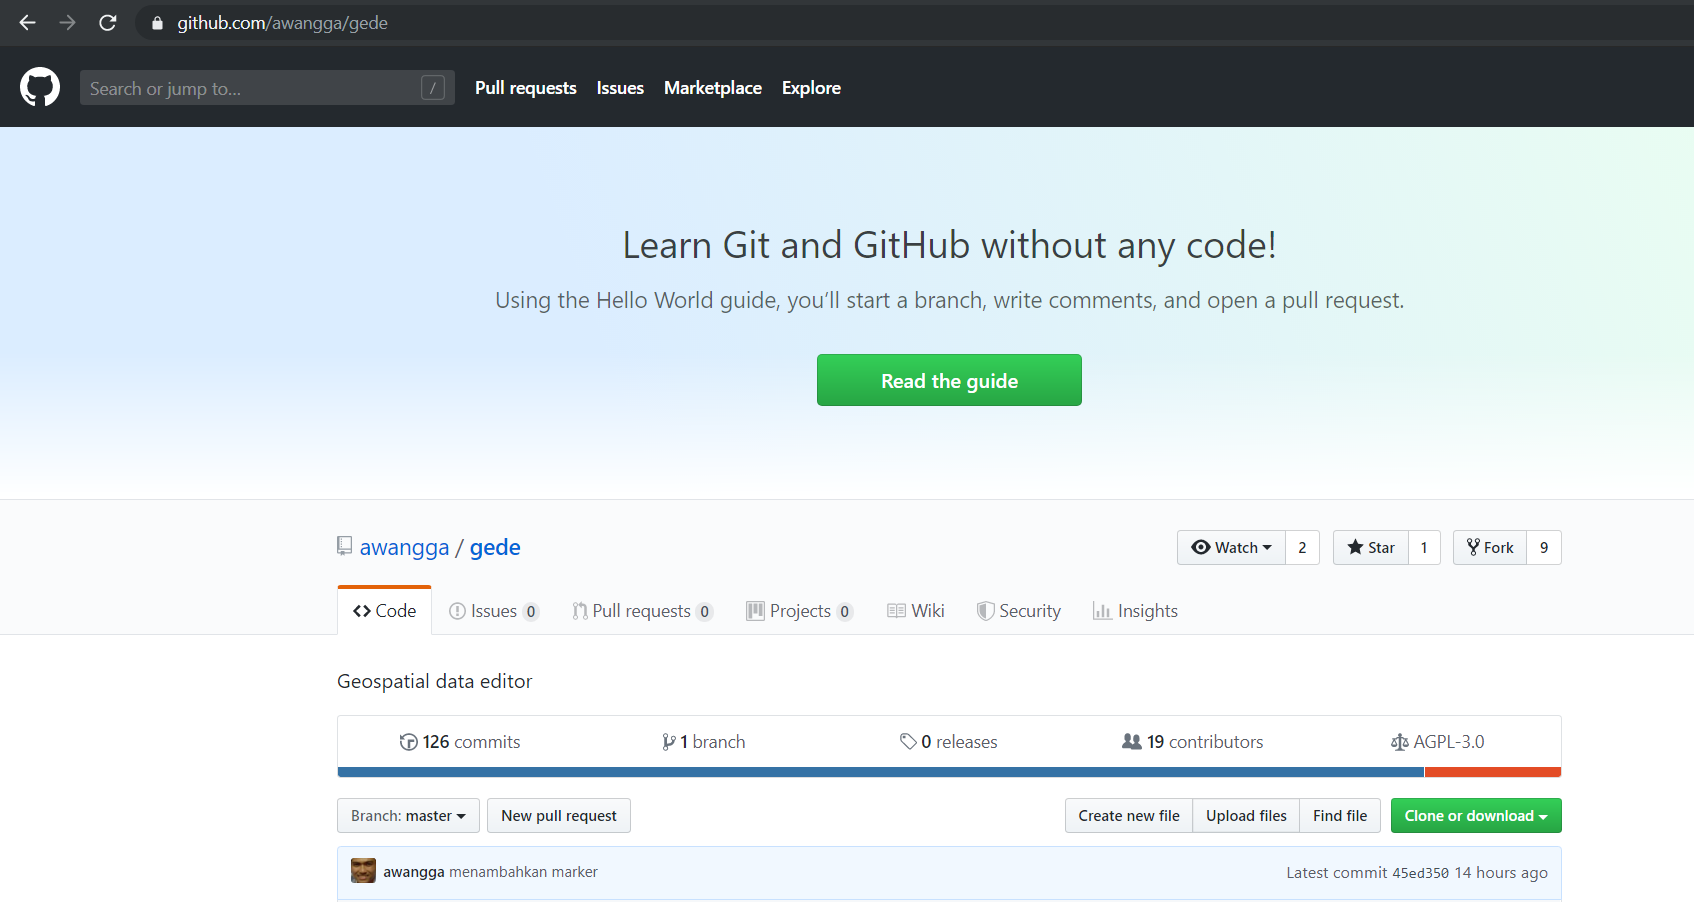
\includegraphics[width=12cm]{figures/1174040/Python3/7.PNG}
		\centering
		\caption{donwload gede}
	\end{figure}
    \item Pindahkan file agm.yml ke dalam folder ms4/Apache/cgi-bin
    \hfill\break
    \begin{figure}[H]
		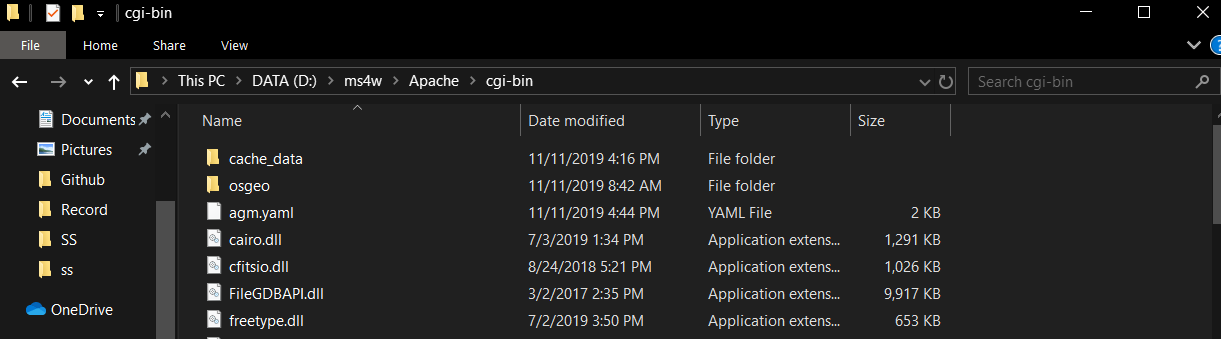
\includegraphics[width=12cm]{figures/1174040/Python3/8.PNG}
		\centering
		\caption{pindahkan agm.yml}
	\end{figure}
    \item Lalu edit directory working dir nya, binary nya, dan map nya sesuai directory kalian
    \hfill\break
    \begin{figure}[H]
		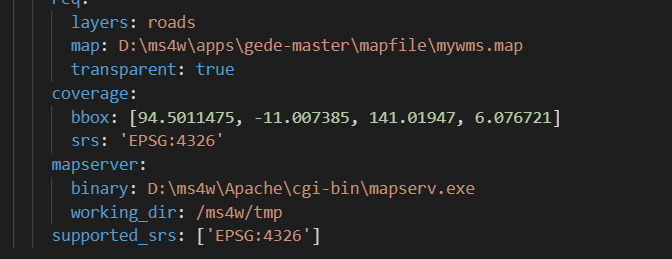
\includegraphics[width=12cm]{figures/1174040/Python3/9.PNG}
		\centering
		\caption{edit directory}
	\end{figure}
    \item buka cmd lalu cd ke folder tadi dan tuliskan seperti di gambar
    \hfill\break
    \begin{figure}[H]
		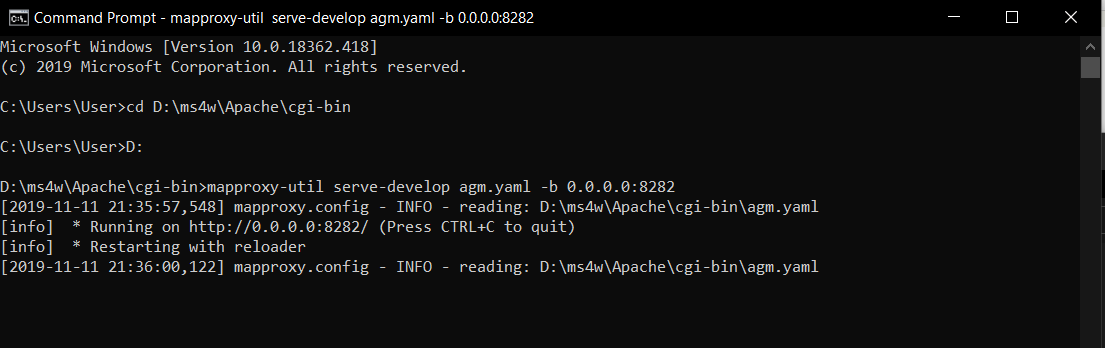
\includegraphics[width=12cm]{figures/1174040/Python3/10.PNG}
		\centering
		\caption{CMD}
	\end{figure}
    \item setelah itu buka browser dan masuk ke dalam apache server tadi
    \hfill\break
    \begin{figure}[H]
		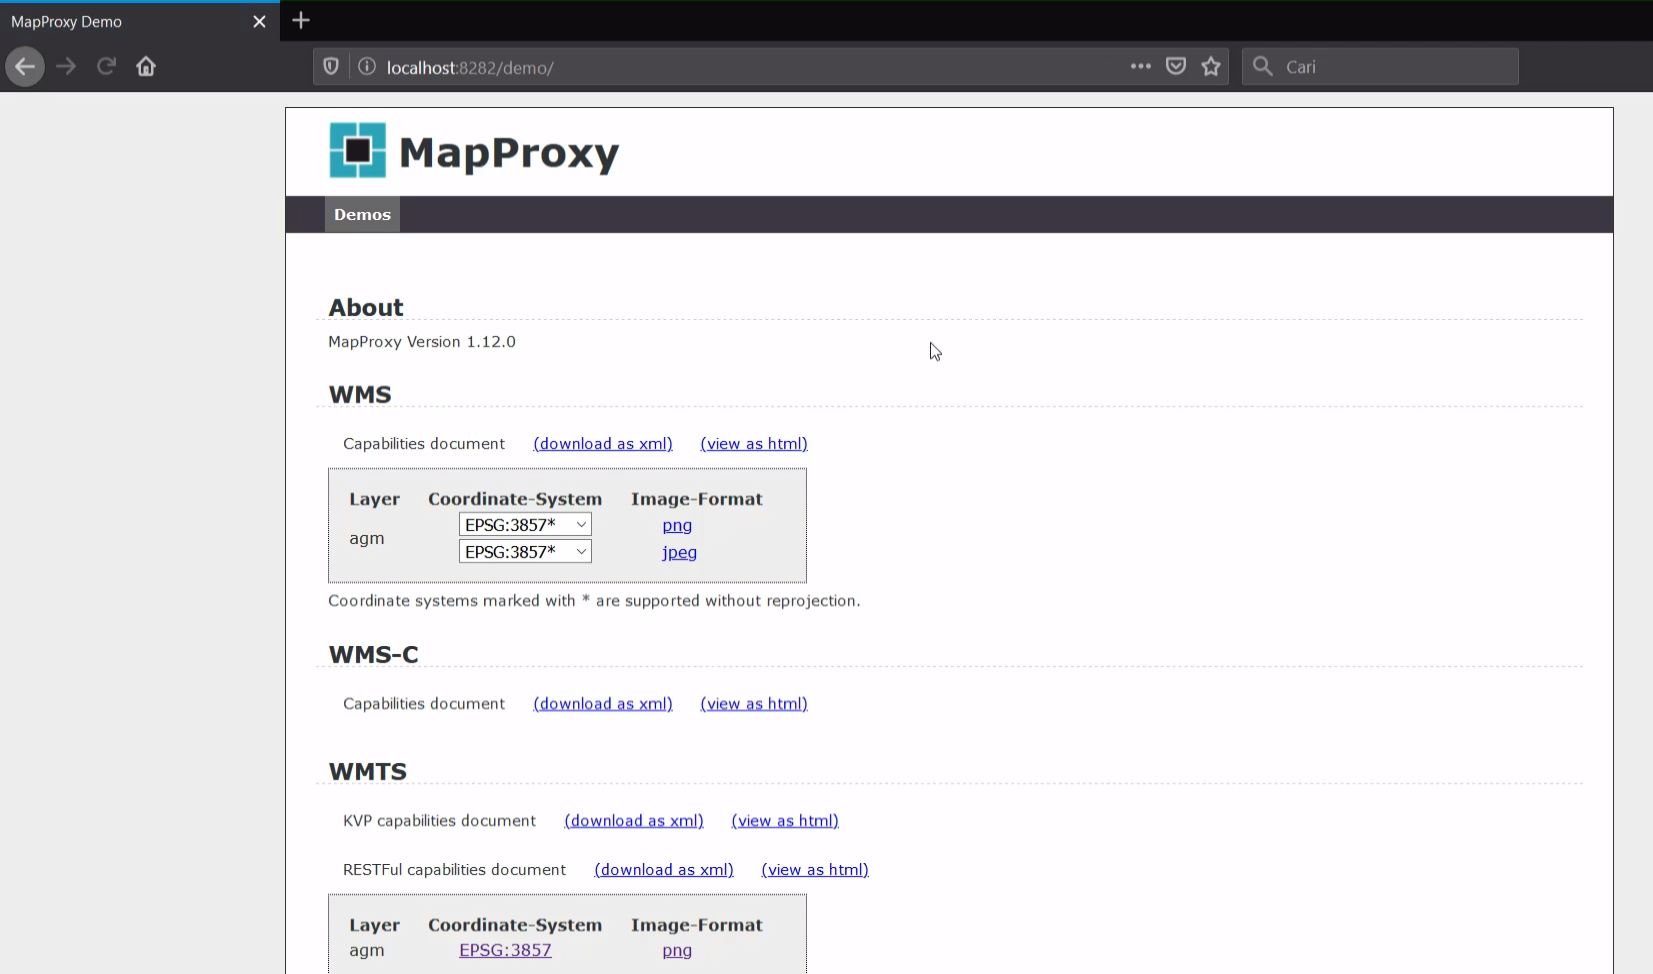
\includegraphics[width=12cm]{figures/1174040/Python3/browser.PNG}
		\centering
		\caption{Hasil}
	\end{figure}
\end{enumerate}    
\subsection{Link Youtube}
\href{https://www.youtube.com/watch?v=8aFRr9DbjQ8}{Yotube Hagan}